\chapter{Internship description}\label{cap:internship-desc}
\intro{This chapter provides an overview of the internship project, including its requirements, goals, and the planning undertaken for the internship period.}
\section{Initial analysis}
The initial phase of the project involved an analysis of the requirements for developing a functional \gls{gang} model. 
This process entailed posing pertinent questions to determine the desired outcomes and the appropriate approach. 
These inquiries encompassed the nature of the generated images, the input image requirements, the network architecture, the extracted image features, and the dataset selection. 
By addressing these questions, the project's requirements, goals, and a comprehensive roadmap were established, laying the foundation for subsequent project execution.
%Given the idea of the project, the first step was to analyze the requirements for get a GAN model that was able to do the job.
%Some questions were made to understand what we want to achieve and how to do it.
%\begin{itemize}
%    \item\textbf{What kind of images the model should generate?}
%    \item\textbf{What kind of images the model should receive as input?}
%    \item\textbf{What kind of network should be used?}
%    \item\textbf{What kind of features should be extracted from the images?}
%    \item\textbf{What kind of dataset should be used?}
%\end{itemize}
%From the previous questions, was possible to define Requirements, Goals and a road-map for the project.\\
\section{Requirements \& Goals}
\subsection{Requirements}
\begin{itemize}
    \item \textbf{Requirement 1}: The dataset used for training the \gls{gang} model must consist of high-quality images of marble slabs to ensure accurate representation;
    \item \textbf{Requirement 2}: The model should possess the capability to generate realistic marble slab images based on given inputs, such as sketches or other forms of guidance;
    \item \textbf{Requirement 3}: The generated images produced by the model should exhibit a high level of quality, comparable to real images of marble slabs, in terms of visual fidelity, texture, and details;
    \item \textbf{Requirement 4}: The generated images should be presented in real time, allowing for immediate visual feedback and preview during the image generation process.
\end{itemize}
\subsection{Goals}
\begin{itemize}
    \item \textbf{Goal 1}: Acquire a diverse and high-quality dataset of marble slab images that encompasses various patterns, colors, and textures to train the \gls{gang} model effectively;
    \item \textbf{Goal 2}: Develop a \gls{gang} model that demonstrates the ability to generate accurate and visually appealing marble slab images from provided inputs, such as sketches or other relevant data;
    \item \textbf{Goal 3}: Create a desktop application that employs the trained \gls{gang} model to generate marble slab images in real time, enabling users to preview the generated images promptly during the image generation process. 
    This application should provide an intuitive user interface for seamless interaction.
\end{itemize}
\section{Planning}
Initially, the project was planned using a story map (See fig.~\ref*{label:story-map}) to define the main features of the project and the main steps to achieve them.
\begin{figure}[H]
    \centering
    \includegraphics[width=1\textwidth]{images/story-map.jpg}
    \caption{Story map}\label{label:story-map}
\end{figure}
\subsection{Road-map}
Following an initial analysis of the story map, it was feasible to establish a project roadmap encompassing the requirements and objectives to be accomplished during the internship period. 
The entire undertaking has been meticulously planned, employing a distinct temporal division across various phases. 
These phases are outlined below:
\begin{itemize}
    \item \textbf{Train period}: This phase entails an in-depth study of the current state of the art and the technologies that will be employed;
    \item \textbf{First period}:  During this phase, the focus will be on image acquisition;
    \item \textbf{Second period}: The primary objective of this period is to augment the dataset by increasing the number of images;
    \item \textbf{Third period}:  In this phase, the key task is to extract the main features;
    \item \textbf{Fourth period}: Network training constitutes the central objective of this Internship;
    \item \textbf{Fifth period}: The final phase involves the analysis of results and the implementation of improvements;
\end{itemize}
%After an Initial analysis of the story map, was possible to define a road-map for the project based on requirements and goals to achieve in the Internship period.
%All the activity has been planned using a specific division of the time in different phases.
%\begin{itemize}
%    \item \textbf{Train period}: study of the state of the art and the technologies that will be used;
%    \item \textbf{First period}: images acquisition;
%    \item \textbf{Second period}: dataset increase, images augmentation;
%    \item \textbf{Third period}: main feature extraction;
%    \item \textbf{Fourth period}: network training;
%    \item \textbf{Fifth period}: results analysis and improvement;
%\end{itemize}
\begin{landscape}
\begin{ganttchart}[%Specs
    y unit title=0.5cm,
    y unit chart=0.6cm,
    x unit=1.0cm,
    vgrid,hgrid,
    title height=1,
%     title/.style={fill=none},
    title label font=\bfseries\footnotesize,
    bar/.style={fill=blue},
    bar height=0.7,
%   progress label text={},
    group right shift=0,
    group top shift=0.7,
    group height=.3,
    group peaks width={0.2},
    inline]{1}{12}
   %labels
   \gantttitle{Internship Project}{12}\\  % title 1           
   \gantttitle{April}{4}                      % title 3
   \gantttitle{May}{4}
   \gantttitle{June}{4}
   % Setting group if any
   \ganttgroup[inline=false]{Train Period}{2}{3}\\ 
   \ganttbar[progress=100,inline=false]{Technology exploration}{2}{3}\\

   \ganttgroup[inline=false]{First Period}{3}{4}\\ 
   \ganttbar[progress=100,inline=false]{Image acquisition}{3}{4}\\
   \ganttmilestone[inline=false]{Milestone 1}{4} \\

   \ganttgroup[inline=false]{Second Period}{3}{4}\\ 
   \ganttbar[progress=100,inline=false]{Dataset improvements}{3}{4}\\
   \ganttmilestone[inline=false]{Milestone 2}{4} \\

   \ganttgroup[inline=false]{Third Period}{4}{5}\\ 
   \ganttbar[progress=100,inline=false]{Features extraction}{4}{5}\\
   \ganttmilestone[inline=false]{Milestone 3}{5} \\

   \ganttgroup[inline=false]{Fourth Period}{5}{7}\\ 
   \ganttbar[progress=100,inline=false]{Network training}{5}{7}\\
   \ganttmilestone[inline=false]{Milestone 4}{7} \\

   \ganttgroup[inline=false]{Fifth Period}{7}{11}\\ 
   \ganttbar[progress=50,inline=false]{General improvements \& Docs}{7}{11}\\
   \ganttmilestone[inline=false]{Milestone 5}{11} \\
\end{ganttchart}
\end{landscape}
\subsection{Study Period:}
This designated period was allocated for an in-depth examination of the current state of the art and the technologies that would be employed throughout the course of the internship. 
The primary focus areas encompassed the following key topics:
\begin{itemize}
    \item \textbf{Machine Learning}: A comprehensive study of the fundamental concepts and principles underpinning machine learning and deep learning;
    \item \textbf{\gls{gang}}: An extensive exploration of the core concepts and functioning principles of GANs;
    \item \textbf{GAN applications}: An examination of the principal applications of \gls{gang}s and their practical utilization;
    \item \textbf{GAN architectures}: A detailed analysis of the primary \gls{gang} architectures and their respective applications;
    \item \textbf{GAN training}: A thorough investigation into the predominant techniques employed for training \gls{gang}s;\@
    \item \textbf{GAN evaluation}: An in-depth exploration of the leading methodologies utilized for evaluating the performance of \gls{gang}s;\@
    \item \textbf{GAN improvements}: A comprehensive study of the key techniques employed to enhance and refine \gls{gang} models;\@
    \item \textbf{GAN applications}:  An exploration of the primary domains where \gls{gang}s find application and their practical implementation;
\end{itemize}
\subsection{First Period:}
During this designated period, the focus was on acquiring images. 
Each Breton machine was already equipped with a camera and a computer featuring specialized software capable of capturing images from the camera. 
The camera captured photographs of each worked slab, which were then transmitted to the database. 
Subsequently, the images were retrieved from the database and stored in a designated folder.
\subsubsection{Challenges:}
The primary challenge encountered during this phase pertained to the quality of the acquired images. 
The machine's image acquisition functionality was not originally intended for use in a machine learning project, resulting in suboptimal image quality. 
The images displayed variations in size, inconsistent backgrounds, and occasionally contained unwanted elements such as light reflections or machine shadows.
\subsubsection{Solutions:}
TTo address these challenges, the following measures were implemented:
\begin{itemize}
    \item \textbf{Background Removal}: To eliminate extraneous elements from the images, a pre-trained machine learning model developed by Breton was employed. 
    This model, in conjunction with the OpenCV library, effectively identified and removed non-slab components from the images, focusing solely on the slabs themselves.
    \item \textbf{Image Defects}: Manual intervention was employed to remove images with light reflections and shadows from the dataset. 
    This task was feasible due to the manageable quantity of such images.
    \item \textbf{Images Resizing}: The images were resized to a standardized dimension while preserving the original aspect ratio.
\end{itemize}
\subsubsection{Milestone:}
At the conclusion of this period, the dataset consisted of 500 images of slabs (See fig.~\ref{fig:slab-sample}), featuring diverse colors and textures. 
The dataset was subsequently divided into two separate parts: one for training purposes and the other for validation, with a split ratio of 70\% for training and 30\% for validation, respectively.
\begin{figure}
    \centering
    \includegraphics[height=6cm]{slabs/intera}
    \caption{Example of a slab}\label{fig:slab-sample}
\end{figure}

\subsection{Second Period:}
During this designated period, the dataset was expanded, and the existing images underwent augmentation techniques.
\subsubsection{Image Augmentation:}
Image augmentation is a technique employed to increase the number of images in a dataset by applying various transformations to the original images. 
This technique proves valuable when the dataset size is insufficient to train a network effectively.
To expand the dataset, each original image was split into smaller images of dimensions 256$\times$256 pixels (See fig.~\ref{fig:slab-split}).
After that the following augmentation techniques were applied to the images:
\begin{itemize}
    \item  \textbf{Resize}: Each image was resized to a larger dimension, increasing from 256$\times$256 pixels to 286$\times$286 pixels;
    \item  \textbf{Random Crop}: A random cropping operation was performed on each image, resulting in a standardized size of 256$\times$256 pixels;
    \item  \textbf{Random Flip}: Each image underwent a random horizontal flipping operation;
\end{itemize}
\subsubsection{Milestone:}
Upon the conclusion of this period, the dataset comprised 7000 images of slabs, exhibiting diverse colors and textures.

\begin{figure}
    \centering
    \includegraphics[width=.24\textwidth]{slabs/crop/crop_0_0}
    \includegraphics[width=.24\textwidth]{slabs/crop/crop_0_1}\\
    \vspace{0.1cm}
    \includegraphics[width=.24\textwidth]{slabs/crop/crop_1_0}
    \includegraphics[width=.24\textwidth]{slabs/crop/crop_1_1}
    \caption{Cropped image}\label{fig:slab-split}
\end{figure}

\subsection{Third Period:}
This designated period was dedicated to identifying the optimal method for extracting features from the images, such as veins, textures, and colors. 
The extraction of features from the images is a critical aspect of the project, as the quality of these features directly impacts the quality of the network. 
Thus, it was imperative to ensure the accuracy of the mask containing the extracted features.

\subsubsection{Vein Extraction:}
Various Python-implemented methods were tested for vein extraction. 
The tested methods included:
\begin{itemize}
    \item \textbf{Thresholding}\footcite{site:opencv-threshold}: This method utilizes the Threshold algorithm, which applies a threshold to the image, retaining only the pixels with values higher than the threshold. 
    To account for varying light conditions across images, the threshold was calculated using the Otsu's method.
    \item \textbf{Canny Edge Detection}\footcite{site:opencv-canny}: This method employs the Canny algorithm, which is an edge detection algorithm utilizing a multi-stage approach to identify edges in images. 
    The algorithm comprises five steps: noise reduction through Gaussian filtering, gradient calculation, non-maximum suppression, double thresholding, and edge tracking by hysteresis. 
    Figure~\ref{fig:canny_compare} illustrates the outcome of Canny Edge Detection
    \begin{figure}[H]
        \centering
        \includegraphics[width=.7\textwidth]{slabs/canny/canny}
        \\
        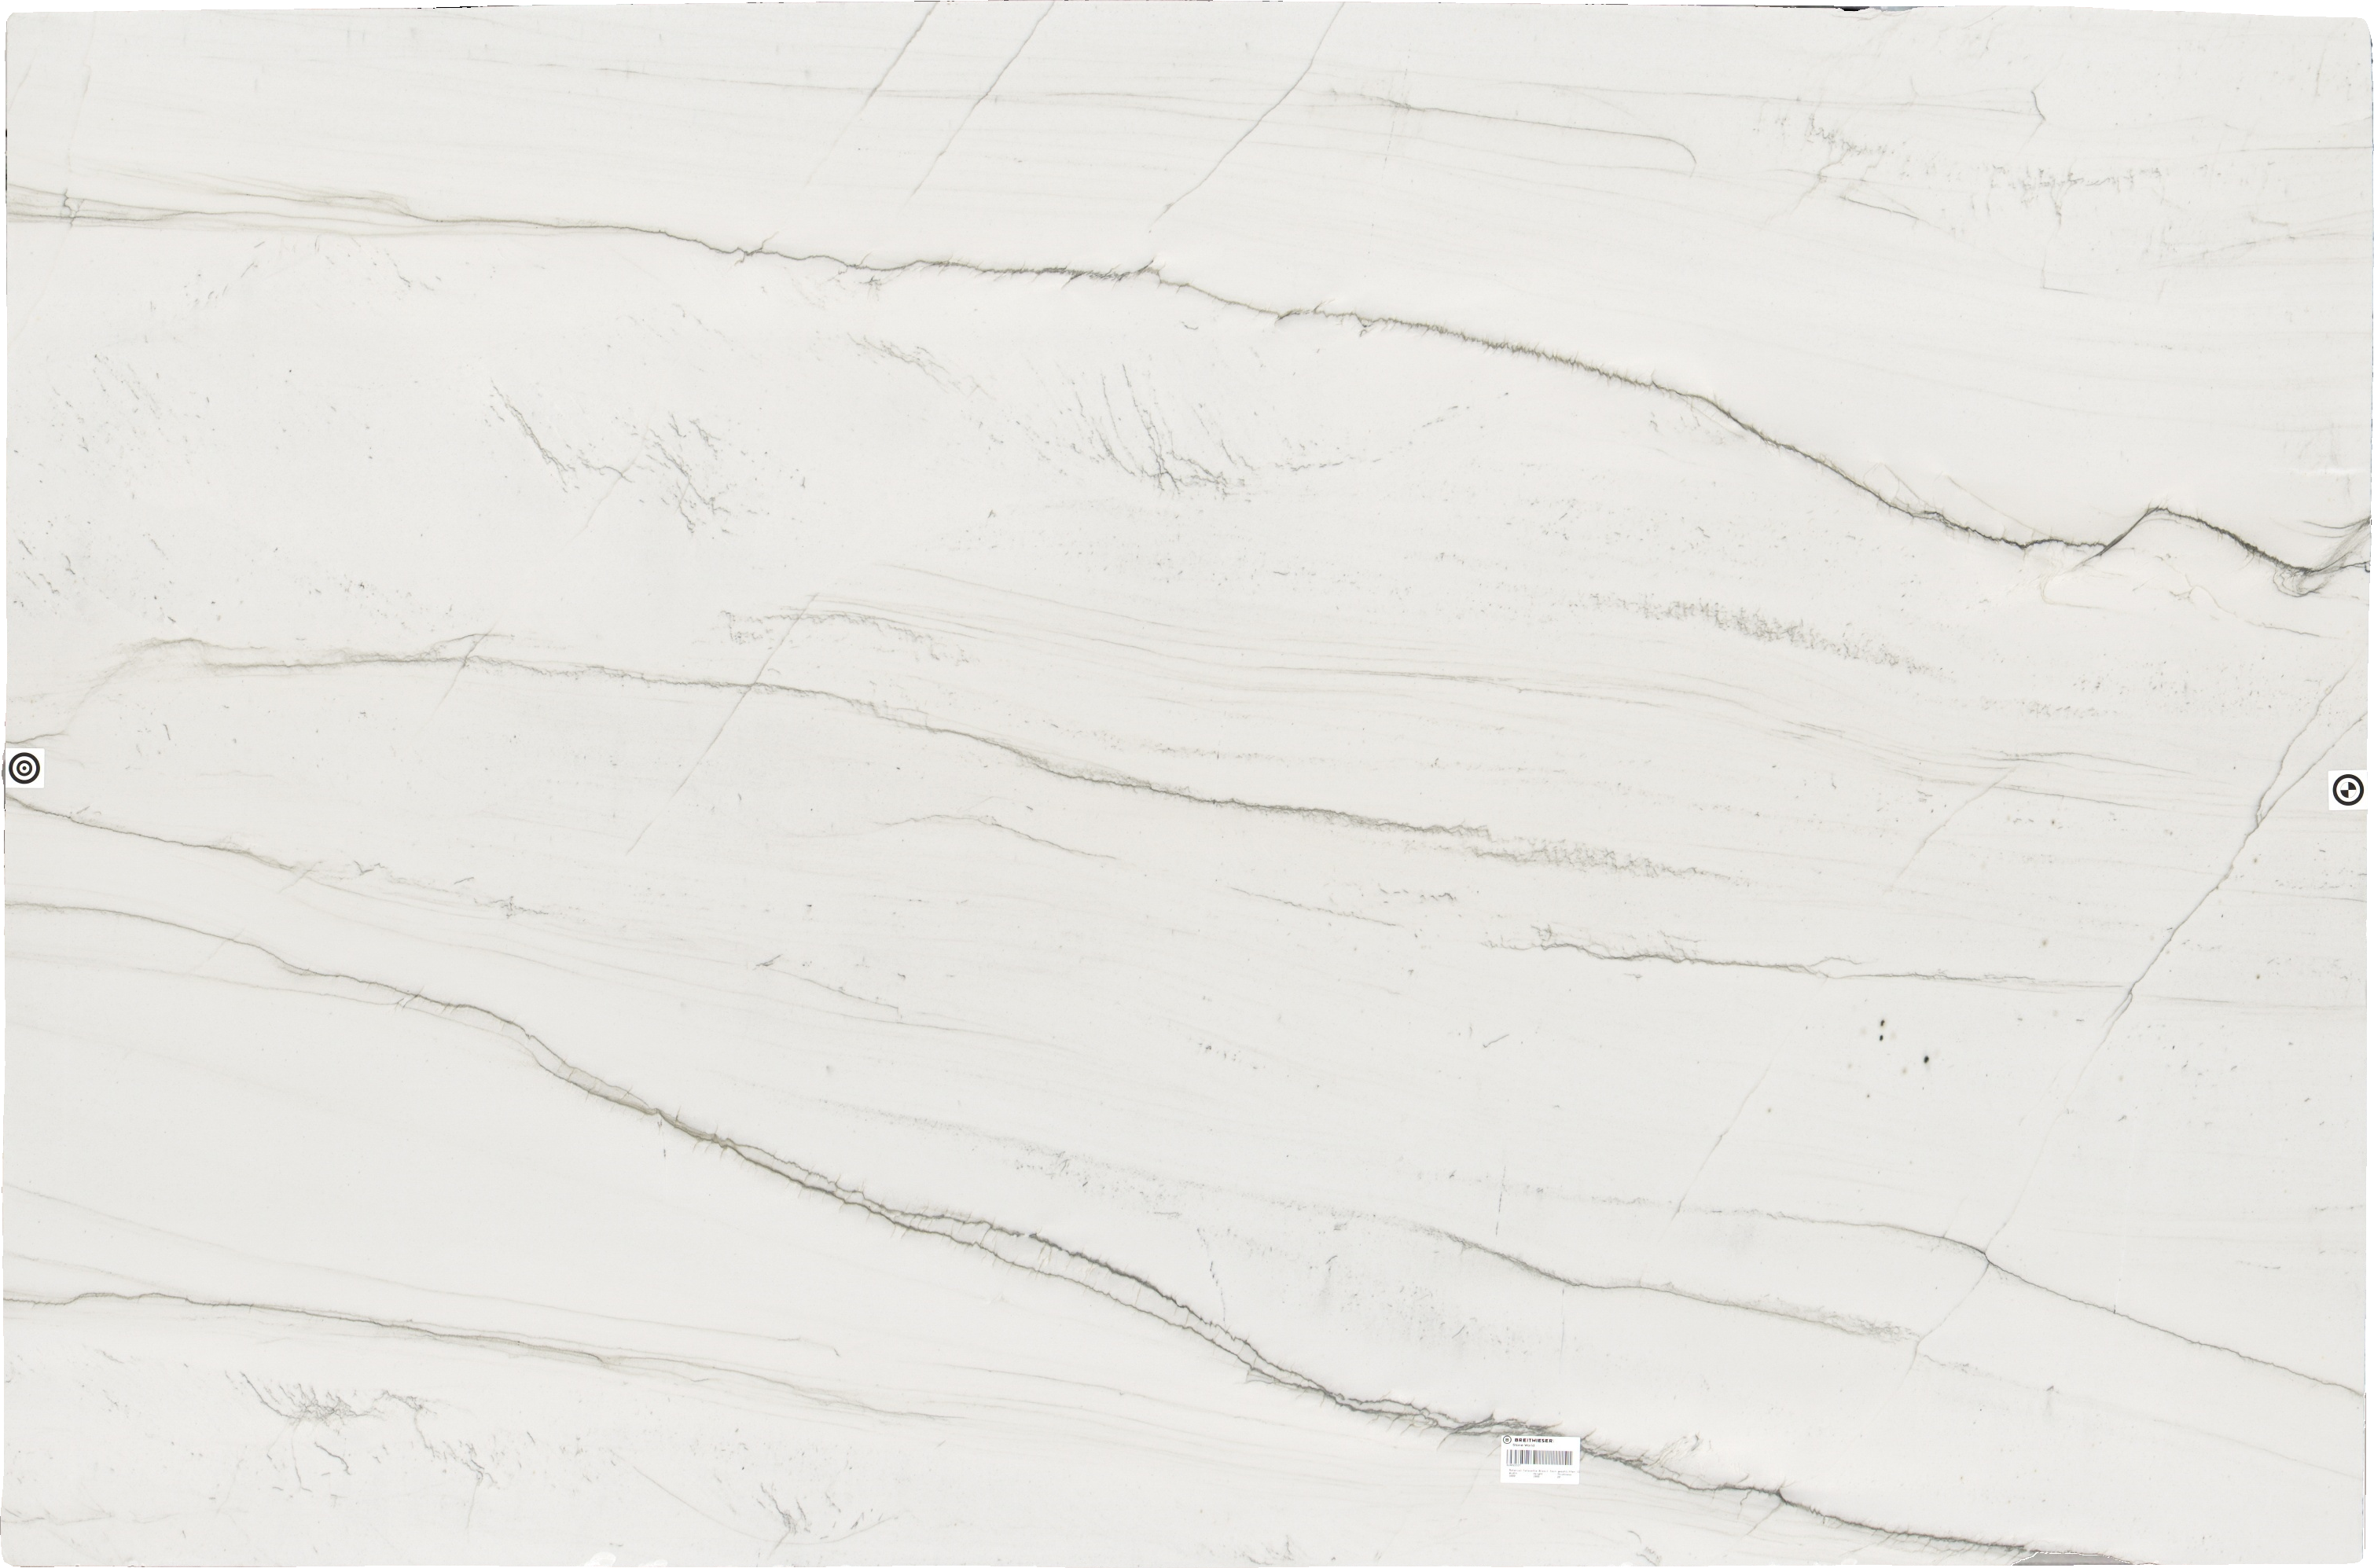
\includegraphics[width=.7\textwidth]{slabs/canny/canny_origin}
        \caption{Canny Edge Detection}\label{fig:canny_compare}
    \end{figure}
    \item \textbf{Meijering \& Contrast filter}\footcite{site:sckit-meijering}: The Meijering filter is based on the Hessian matrix, which calculates the second-order partial derivatives of a function. 
    Eigenvalues and eigenvectors obtained from the Hessian matrix enable the identification of line-like structures in the image. 
    The contrast filter is employed to enhance image contrast. 
    Figure~\ref{fig:meij_compare} presents the result of the Meijering \& Contrast filter.
    \begin{figure}[H]
        \centering
        \includegraphics[width=.7\textwidth]{slabs/meijering/meije}
        \\
        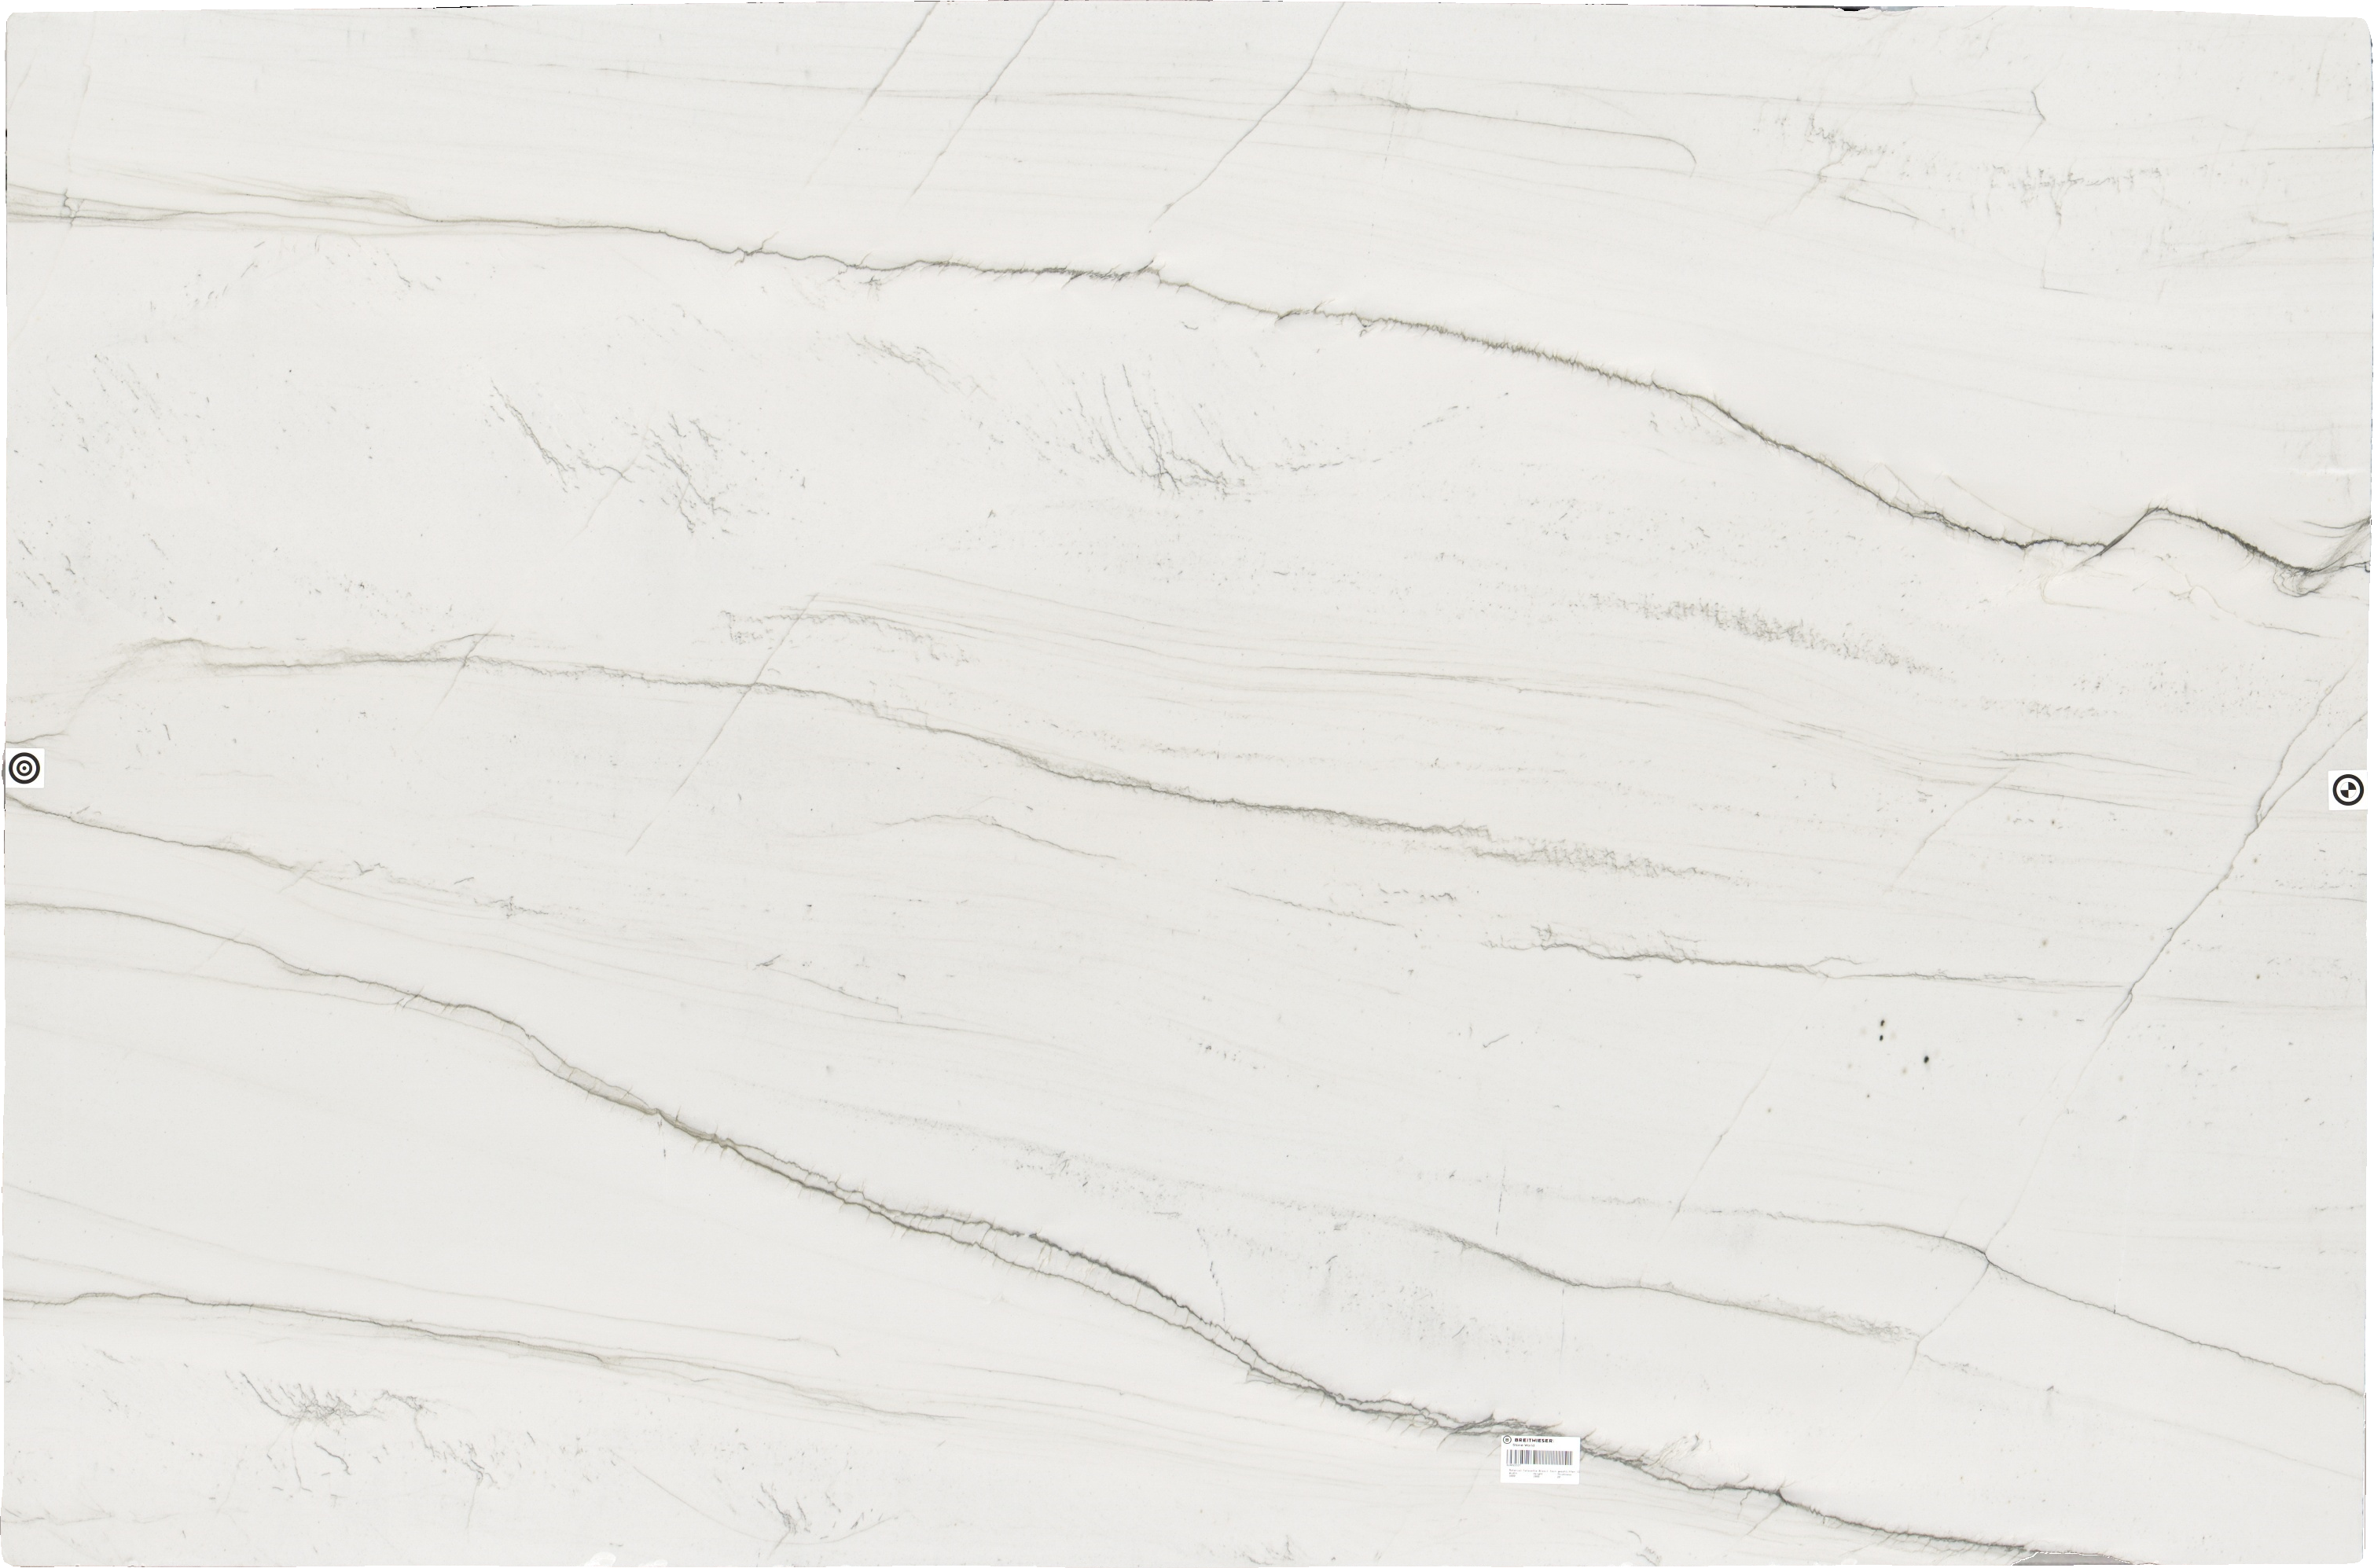
\includegraphics[width=.7\textwidth]{slabs/canny/canny_origin}
        \caption{Meijering \& Contrast filter}\label{fig:meij_compare}
    \end{figure}
    \item \textbf{HED (Holistically-Nested Edge Detection)}\footcite{paper:hed}: This method is based on the \gls{HEDG}\glsfirstoccur algorithm, which employs a deep neural network for edge detection in images. 
    The algorithm involves three steps: utilizing a pre-trained network to extract features from the image, applying a multi-scale algorithm to extract edges from the features, and linking the edges using the Canny algorithm. 
    Figure~\ref{fig:hed_compare} showcases the result of the \gls{HEDG} algorithm.
    \begin{figure}[H]
        \centering
        \includegraphics[width=.7\textwidth]{slabs/hed/hed}
        \\
        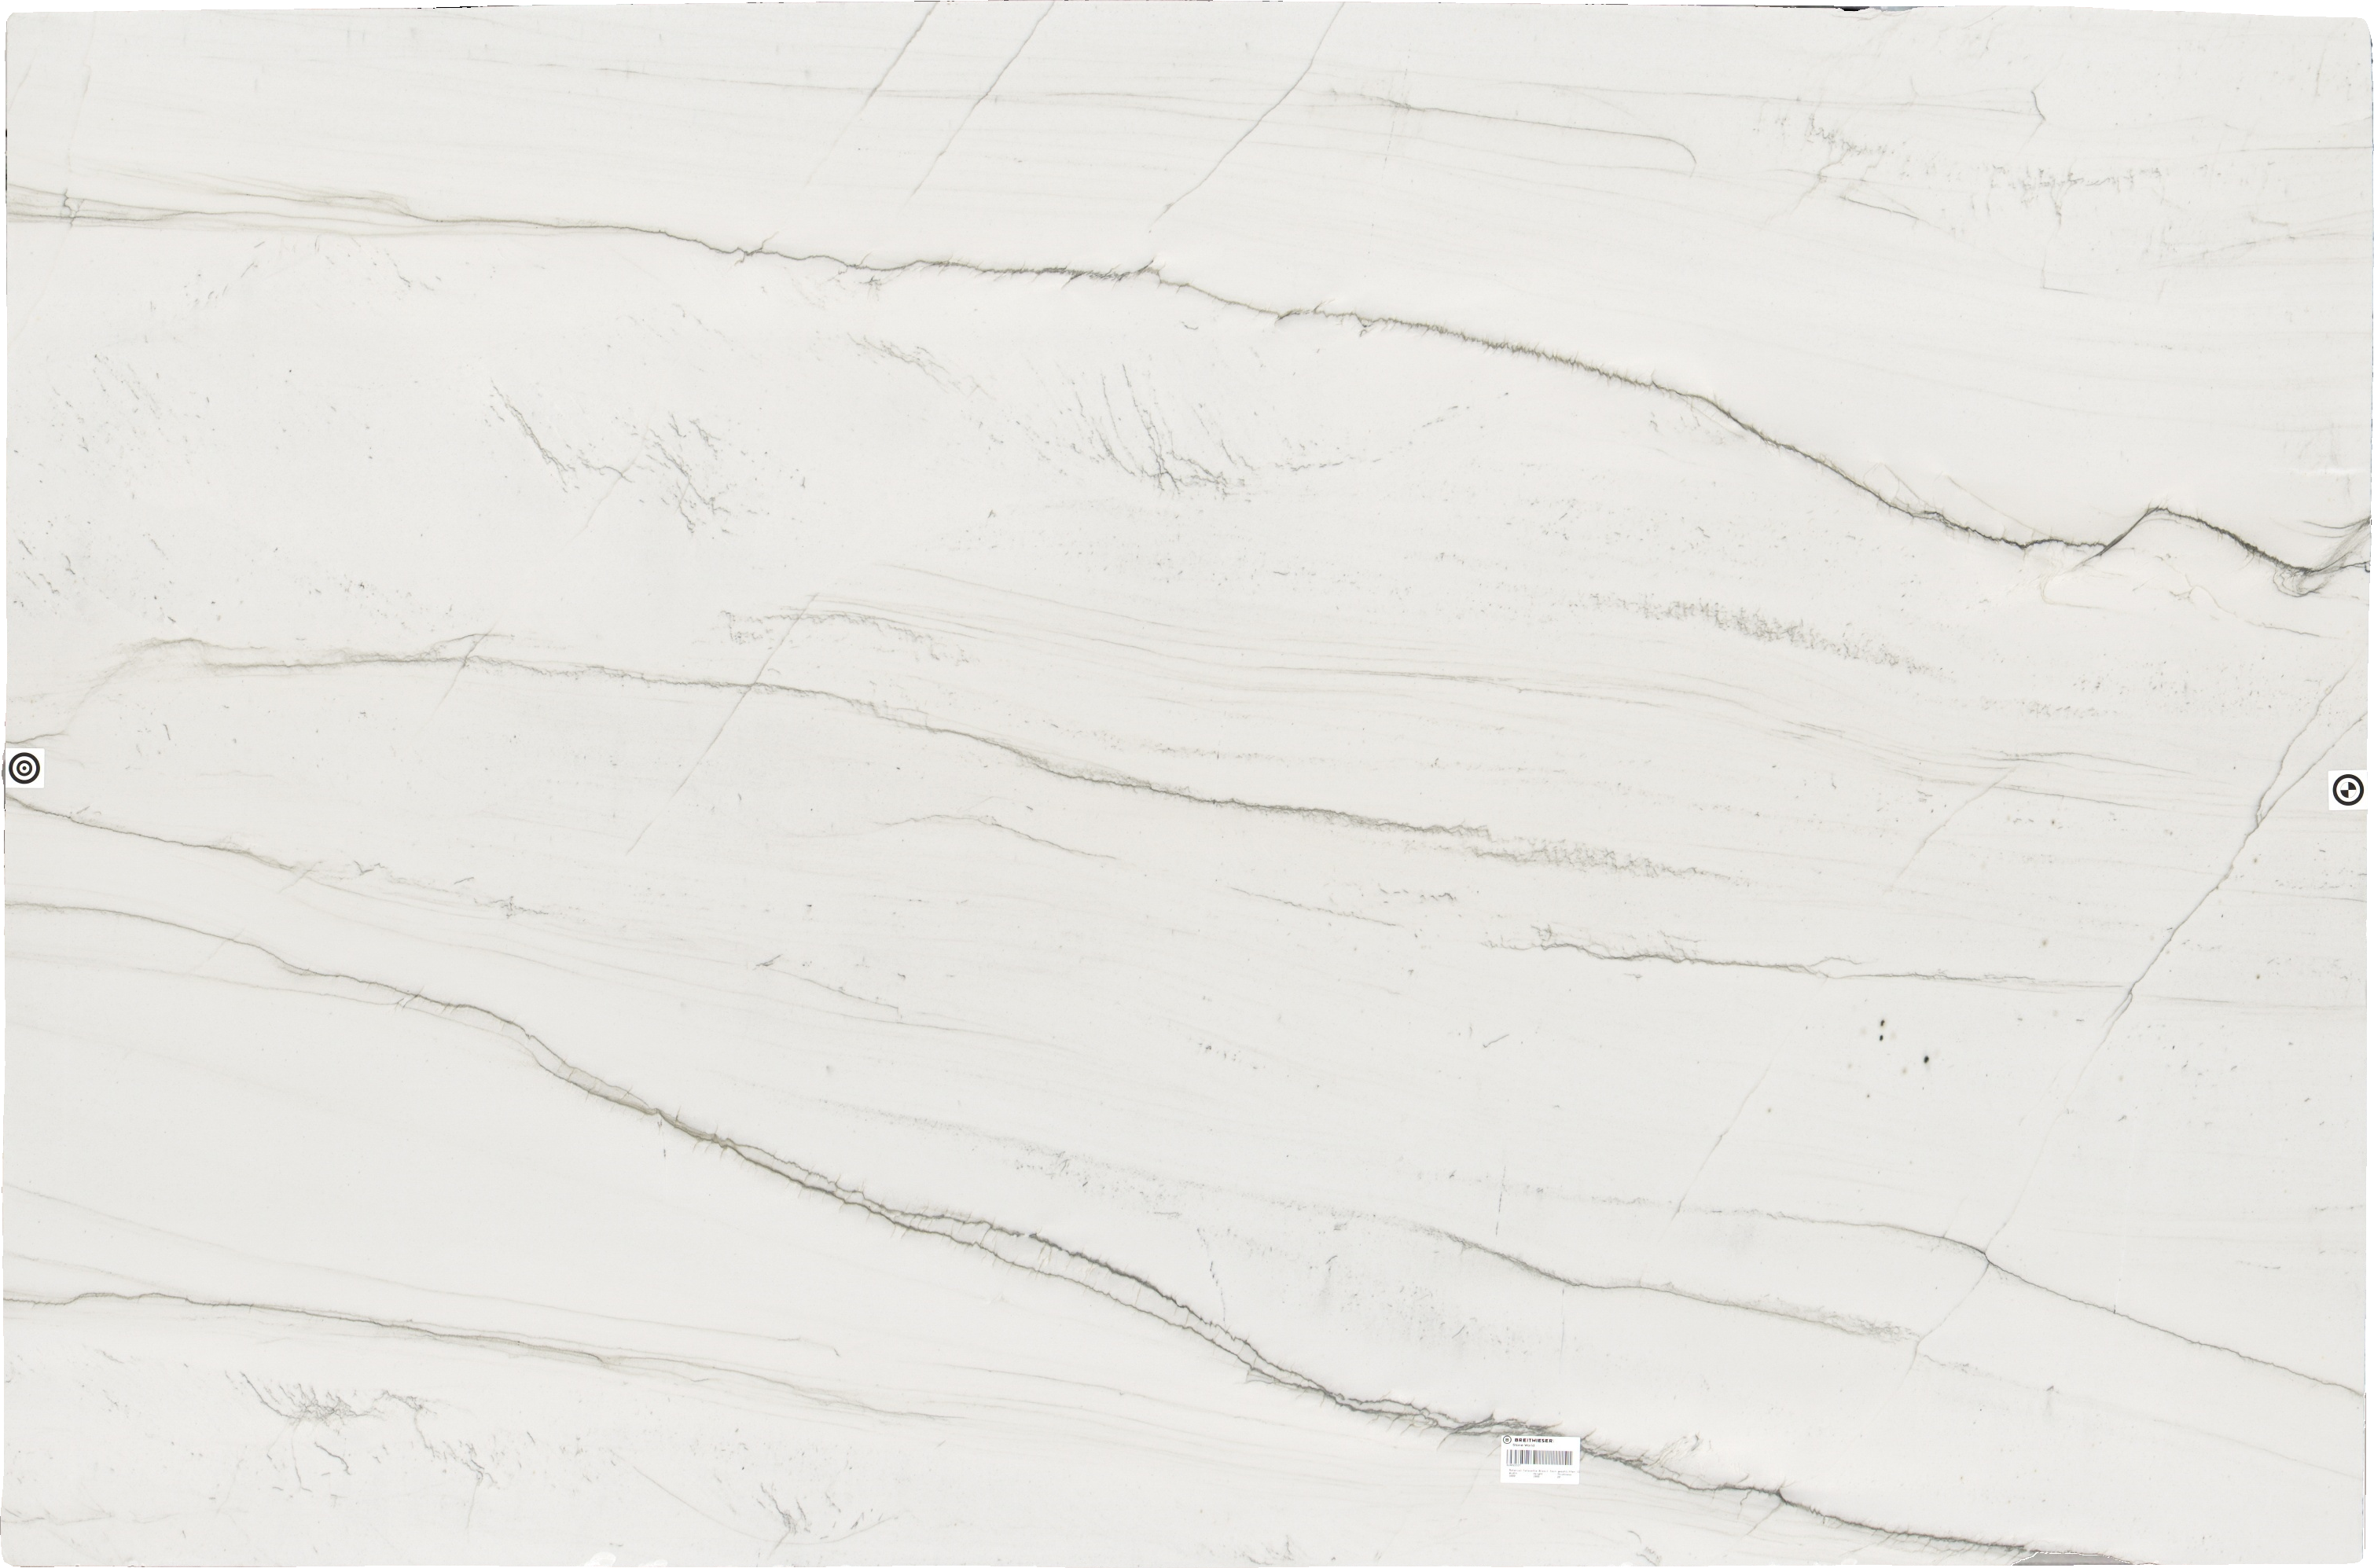
\includegraphics[width=.7\textwidth]{slabs/canny/canny_origin}
        \caption{HED}\label{fig:hed_compare}
    \end{figure}
\end{itemize}
\subsubsection{Milestone:}
At the conclusion of this period, the results indicated that the Meijering \& Contrast filter and the Canny Edge Detection methods were the most effective. 
The \gls{HEDG} method was discarded due to its sluggish performance and subpar results, often introducing noise in the form of random lines into the images. 
The two preferred methods successfully extracted the vein structures from the images, considering that an unsupervised approach was employed.
\subsubsection{Improvements:}
One potential avenue for improvement involves the utilization of a supervised method for vein extraction. 
This method would offer greater accuracy compared to unsupervised methods, as it would be trained specifically for vein extraction. 
However, implementing a supervised approach necessitates significant time and a substantial number of hand-labeled images to train the model effectively.

\subsection{Fourth Period:}
During this designated period, the focus was on training the network. 
The network employed for this purpose was a pix2pix network, which utilizes a Conditional Generative Adversarial Network (\gls{cgang}) to generate images. 
The training process involved utilizing the dataset created in the preceding periods and the hardware resources provided by the company (See~\ref{subsec:hardware})

Various configurations of the network were tested during this period, involving the fine-tuning of hyperparameters to identify the optimal setup. 
The specific configuration details of the network will be elaborated upon in Chapter~\ref{cap:design-coding}.
\subsubsection{Milestone:}
Upon the conclusion of this period, the network demonstrated its capability to generate images of slabs exhibiting a diverse range of colors and textures (See~\ref*{fig:gen-images}).
%list of img generated
\begin{figure}
    \centering
    \includegraphics[width=.7\textwidth]{slabs/generated/amogus}
    \\
    \includegraphics[width=.7\textwidth]{slabs/generated/breton}
    \\
    \includegraphics[width=.7\textwidth]{slabs/generated/slab}
    \caption{Generated images}\label{fig:gen-images}
\end{figure}